\documentclass[12pt,letterpaper]{article}

\usepackage{amsmath}
%\usepackage[margin=1.3in]{geometry}
\usepackage[pdftex]{graphicx}
\usepackage{hyperref} 

\parindent 0cm

\graphicspath{{figures/}}

\author{
    Jed Barlow\\
    \textit{jbarlow@lavabit.com}
}
\title{SeqPartitioner Geneious Plugin Manual}

\begin{document}
\maketitle

\hfill

%\newpage
\tableofcontents

\newpage
\section{Overview}

SeqPartitioner is a Geneious plugin for partitioning allele multisets.  The
plugin operates on alignments to produce various tables expressing the grouping
of equivalent aligned nucleotide sequences and the number of differences
between strains in terms of non-equivalent alleles.

\section{Installation}
The plugin can be obtained, at the time of the writing of this manual, from two
locations.

\begin{itemize}
\item
    In source form: \url{http://github.com/jedbarlow/biol398\_seq\_partitioner/}
\item
    As a compiled package: \url{http://www.ualberta.ca/~ejbarlow/biol398/}
\end{itemize}

Once obtained, the plugin \textit{SeqPartitioner.gplugin} can be installed by
navigating the Geneious menu to \texttt{Tools->Plugins}.

\hfill

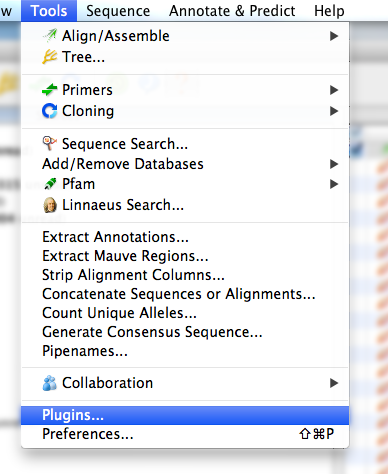
\includegraphics[resolution=130]{menu_entry_plugins.png}

\hfill

Then pressing the \texttt{Install plugin from a gplugin file...} button.

\hfill

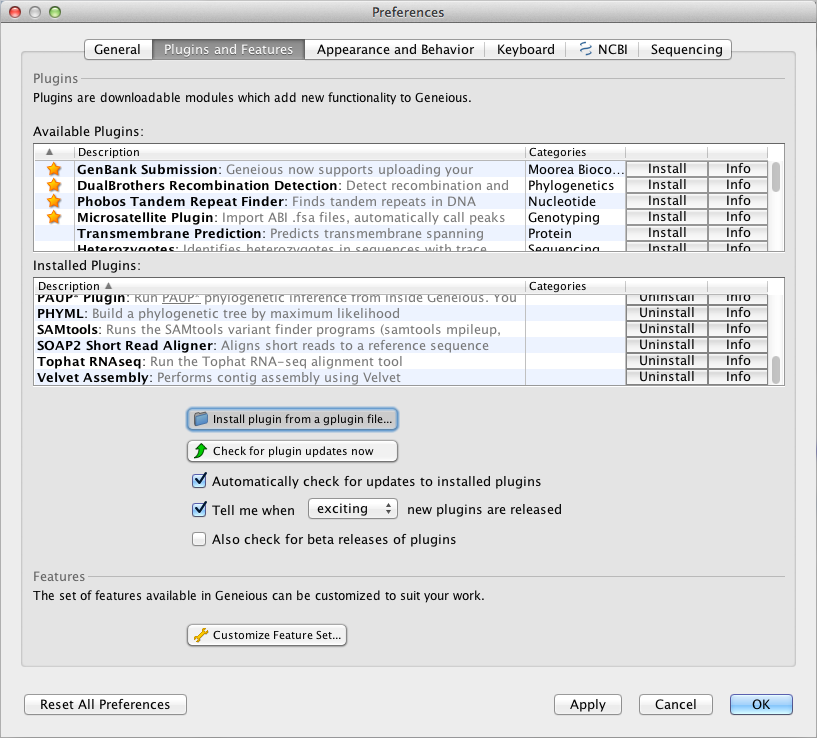
\includegraphics[resolution=130]{plugins_dialog.png}

\hfill

Finally, navigate to and select the file plugin package file
\textit{SeqPartitioner.gplugin}.

Once installed, an entry should appear in the Geneious menu as shown in a figure
below.

\section{Operation}
The plugin is used by first selecting a set of alignments.

\hfill

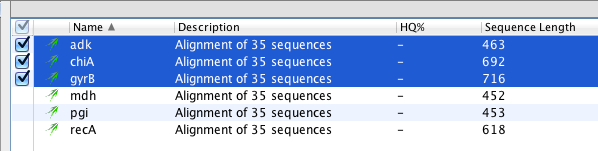
\includegraphics[resolution=120]{alignment_selection.png}

\hfill

Then navigating the menu to \texttt{Tools->Partition Allele Multiset}.


\hfill

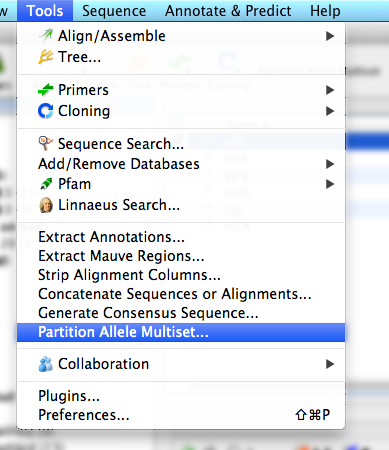
\includegraphics[resolution=130]{menu_entry.png}

\hfill

Then choosing options in the dialog box.

\hfill

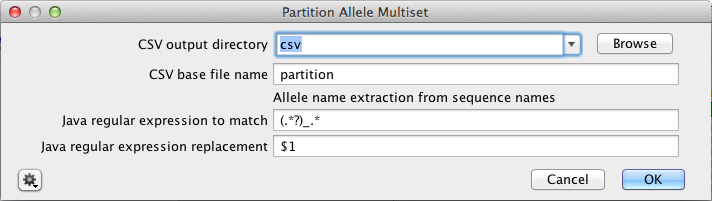
\includegraphics[resolution=130]{dialog_box.png}

\hfill

The meanings of the fields are as follows:

\begin{itemize}
\item \textit{CSV output directory} \hfill \\
\addcontentsline{toc}{subsubsection}{CSV output directory}
    This is the target directory into which the resulting table files will be
    written.  Note that pre-existing files of the same name as the output files
    will be overwritten without warning or prompting.

\item \textit{CSV base file name} \hfill \\
\addcontentsline{toc}{subsubsection}{CSV base file name}
    This is a string of text which will be appended with descriptive suffixes
    for each table.  For example the following entry,
    
    \begin{itemize}
    \item[]\texttt{partition1}
    \end{itemize}

    will result in the production of files such as these two,

    \begin{itemize}
    \item[]\texttt{partition1\_gene\_vs\_strain.csv}
    \item[]\texttt{partition1\_strain\_vs\_strain.csv}
    \item[]\texttt{partition1\_strain\_vs\_strain\_matrix.csv}
    \end{itemize}

\item \textit{Java regular expression to match} \hfill \\
\addcontentsline{toc}{subsubsection}{Java regular expression to match}
    The purpose of these last two fields is to establish a transformation of
    each sequence name so that allele's are grouped together under the name of
    a gene.  The first field is a pattern to match against each sequence name.
\item \textit{Java regular expression replacement} \hfill \\
\addcontentsline{toc}{subsubsection}{Java regular expression replacement}
    This field describes a replacement for the text in the sequence name
    matched by the pattern in the previous field.


\end{itemize}

\subsection{Example Regular Expressions}

\begin{itemize}
\item
    If for example, the names of the sequences are patterned as
    \texttt{[GENE]\_[STRAIN]}, then the default entry will work correctly by
    grouping all strains for each gene together under the name of the gene.

    Pattern: \texttt{(.*?)\_.*}

    Replacement: \texttt{\$1}

    The period matches any character, and the star matches a sequence of
    characters matching the previous construct (the period in this case).  The
    question mark indicates that the star should only match until the next
    construct (an underscore in this case) can be matched.  The parenthesis in
    the pattern designate the inner matching text as an identifiable string
    which can be referred to in the replacement as \texttt{\$1}.  It is
    important to note that text in the sequence name which does not match the
    pattern will be left unmodified, so the last part of the pattern
    \texttt{\_.*}, which matches the \texttt{\_[STRAIN]} portion of the name,
    cannot be omitted.

\item
    Sequence names patterned such as \texttt{[STRAIN]\_[GENE]} can be properly
    grouped by slightly modifying the pattern in the above.

    Pattern: \texttt{.*?\_(.*)}

    Replacement: \texttt{\$1}

\end{itemize}

More information about regular expressions, and regular expressions in
Java, can be found at the following urls.
\begin{itemize}
\item
    \url{https://en.wikipedia.org/wiki/Regular\_expression}
\item
    \url{http://docs.oracle.com/javase/tutorial/essential/regex/intro.html}
\item
    \url{http://docs.oracle.com/javase/7/docs/api/java/util/regex/Pattern.html}
\end{itemize}

\newpage
\section{Description of Output Tables}

Two tables are created when the plugin is run.  The tables with the suffixes
\texttt{\_straing\_vs\_strain} and \texttt{\_straing\_vs\_strain\_matrix}
describe the number of different alleles (according to the equivalence
relation) between two 

    %TODO: describe how broken equivalence relations are handled.

\end{document}


% Each alignment file is assumed to contain sequences pertaining to exactly one
% gene, and it is assumed that each gene has all it's sequences in one
% alignment file.

% The purpose of the regexp is to enable strains to be correlated accross
% alignment files
